\section{Область устойчивости}
Рассмотрим структурную схему третьего порядка, представленную на рисунке \ref{fig:scheme2}.

\begin{figure}[ht!]
    \centering
    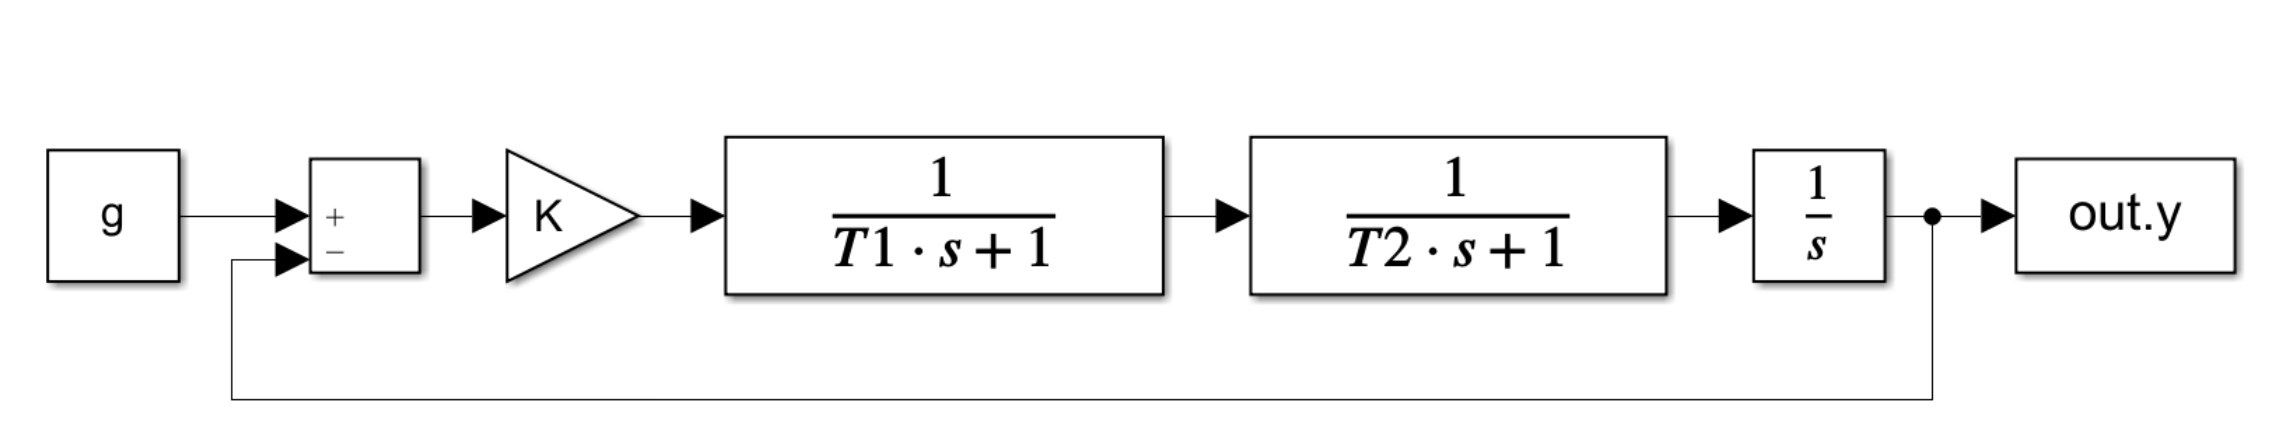
\includegraphics[width=\textwidth]{media/scheme2.png}
    \caption{Схема моделирования}
    \label{fig:scheme2}
\end{figure}

\subsection{Передаточная функция}

Рассмотрим передаточную функцию $T_{12}$, получающуюся в результате последовательного соединения 
передаточных функций $T_1$ и $T_2$. В таком случае передаточная функция $T_{12}$ будет равна 
произведению передаточных функций $T_1$ и $T_2$.
\begin{equation}
    T_{12} = T_1 \cdot T_2 = \frac{1}{T_1p + 1} \cdot \frac{1}{T_2p + 1} 
\end{equation}

Полюсами передаточной функции называются корни характеристического полинома ее знаменателя. 
\begin{equation}
    (T_1\lambda + 1)(T_2\lambda + 1) = 0
\end{equation}
Таким образом, решая систему уравнений, получим искомые коэффициенты $T_1$ и $T_2$, при 
которых полюса передаточной функции $T_{12}$ будут соответствовать значениям $\lambda_1$ и $\lambda_2$.
\begin{equation}
    \begin{cases}
        T_1\lambda_1 + 1 = 0 \\
        T_2\lambda_2 + 1 = 0
    \end{cases} \Rightarrow
    \begin{cases}
        T_1 = \frac{-1}{\lambda_1} \\
        T_2 = \frac{-1}{\lambda_2}
    \end{cases} \Rightarrow
    \begin{cases}
        T_1 = \frac{-1}{-5.5} = \frac{2}{11} \\ 
        T_2 = \frac{-1}{-6} = \frac{1}{6}
    \end{cases}
    \label{eq:T1T2}
\end{equation}


\subsection{Переход от схемы к уравнению} 
Запишем передаточную функцию для схемы на рисунке \ref{fig:scheme2}:
\begin{equation}
    W_{123}(p) = K \cdot \frac{1}{T_1p + 1} \cdot \frac{1}{T_2p + 1} \cdot \frac{1}{p}
\end{equation}
Так как система имеет отрицательную обратную связь, то передаточная функция замкнутой системы 
будет равна:
\begin{equation}
    W(p) = \frac{W_{123}}{1 + W_{123}\cdot 1} = \frac{\dfrac{K}{T_1T_2p^3 + (T_1 + T_2)p^2 + p}}{\dfrac{K}{T_1T_2p^3 + (T_1 + T_2)p^2 + p} + 1} = \frac{K}{T_1T_2p^3 + (T_1 + T_2)p^2 + p + K}
\end{equation}
\begin{equation}
    y(t) = W(p)u
\end{equation}
Запишем систему в операторном виде:
\begin{equation}
    y = \frac{K}{T_1T_2p^3 + (T_1 + T_2)p^2 + p + K} \cdot g
    \notag
\end{equation}
\begin{equation}
    T_1T_2p^3 y + (T_1 + T_2)p^2 y + p y + Ky = K^2 g
\end{equation}
И в виде дифференциального уравнения:
\begin{equation}
    T_1T_2 \dddot{y} + (T_1 + T_2) \ddot{y} + \dot{y} + Ky = K^2 g
\end{equation}
Для определения устойчивости рассмотрим свободное движение системы, то есть $g = 0$.
\begin{equation}
    T_1T_2 \dddot{y} + (T_1 + T_2) \ddot{y} + \dot{y} + Ky = 0
    \label{eq:system2}
\end{equation}
\subsection{Критерий Гурвица}
Согласно критерию Гурвица, система находится на границе устойчивости, если $a_n > 0$ и $\Delta_{n - 1}=0$ а все
остальные миноры $\Delta_1,~\Delta_2,\cdots\Delta_{n-2}$ положительны.
Где $\Delta_i$ -- угловой минор матрицы $A$ размера $i$.  Если все угловые миноры положительны, то система
ассимптотически устойчива.
\begin{equation}
    A = \begin{bmatrix}
        a_{n-1} & a_{n-3} & a_{n-5} & \cdots & 0 \\
        a_n & a_{n-2} & a_{n-4} &\cdots & 0\\
        0 & a_{n-1} & a_{n-3} & \cdots & 0\\
        0 & a_n & a_{n-2} & \cdots & 0 \\
        \vdots & \vdots & \vdots & \ddots & \vdots \\
        0 & 0 & 0 & \cdots & a_0
    \end{bmatrix}
\end{equation}
где $a_0,\ldots a_n$ - коэффициенты дифференциального уравнения.
Для уравнения третьего порядка:
\begin{equation}
    A = \begin{bmatrix}
        a_2 & a_0 & 0 \\
        a_3 & a_1 & 0 \\
        0 & a_2 & a_0
    \end{bmatrix}
\end{equation}
где $a_0,\ldots a_3$ - коэффициенты дифференциального уравнения.
В нашем случае:
\begin{equation}
    \begin{cases}
        a_3 > 0 \\ 
        a_2 > 0 \\ 
        \begin{vmatrix}
            a_2 & a_0 \\
            a_3 & a_1
        \end{vmatrix} > 0 \\ 
        \begin{vmatrix}
            a_2 & a_0 & 0 \\
            a_3 & a_1 & 0 \\
            0 & a_2 & a_0
        \end{vmatrix} = 0
    \end{cases}
\end{equation}

\begin{equation}
    \begin{cases}
        a_3 > 0 \\ 
        a_2 > 0 \\   
        a_2a_1 - a_3a_0 > 0 \\
        a_0a_1a_2 - a_3a_0^2 = 0
    \end{cases}
\end{equation}
Пологая $a_3 = 1$, можно упростить систему до: 
\begin{equation}
    \begin{cases}
        a_0, a_1, a_2 > 0 \\ 
        a_1a_2 = a_0
    \end{cases}
\end{equation}
для границы устойчивости и 
\begin{equation}
    \begin{cases}
        a_0, a_1, a_2 > 0 \\ 
        a_1a_2 > a_0
    \end{cases}
\end{equation}
для асимптотической устойчивости.

Перепишем уравнение \ref{eq:system2} в соответствии с принятым $a_3 = 1$:
\begin{equation}
    \dddot{y} + \frac{T_1 + T_2}{T_1T_2} \ddot{y} + \frac{1}{T_1T_2} \dot{y} + \frac{K}{T_1T_2}y = 0
\end{equation} 
Получим систему:
\begin{equation}
    \begin{cases}
        \frac{K}{T_1T_2} > 0 \\
        \frac{1}{T_1T_2} > 0 \\ 
        \frac{T_1 + T_2}{T_1T_2} > 0 \\ 
        \frac{T_1 + T_2}{T_1^2T_2^2} \ge \frac{K}{T_1T_2} \\ 
    \end{cases}
\end{equation}
Фиксируя $T_2 > 0$, получим: 
\begin{equation}
    \begin{cases}
        K > 0 \\
        T_1 > 0 \\ 
        \frac{T_1 + T_2}{T_1T_2} \ge K \\ 
    \end{cases}
\end{equation}
Фиксируя $T_1 > 0$, получим: 
\begin{equation}
    \begin{cases}
        K > 0 \\
        T_2 > 0 \\  
        \frac{T_1 + T_2}{T_1T_2} \ge K \\ 
    \end{cases}
\end{equation}
Графики решений уравнений при вычисленных $T_1,~T_2$ (см. \ref{eq:T1T2}) приведены на рис. \ref{fig:T1K}, \ref{fig:T2K}.

\begin{figure}
    \centering
    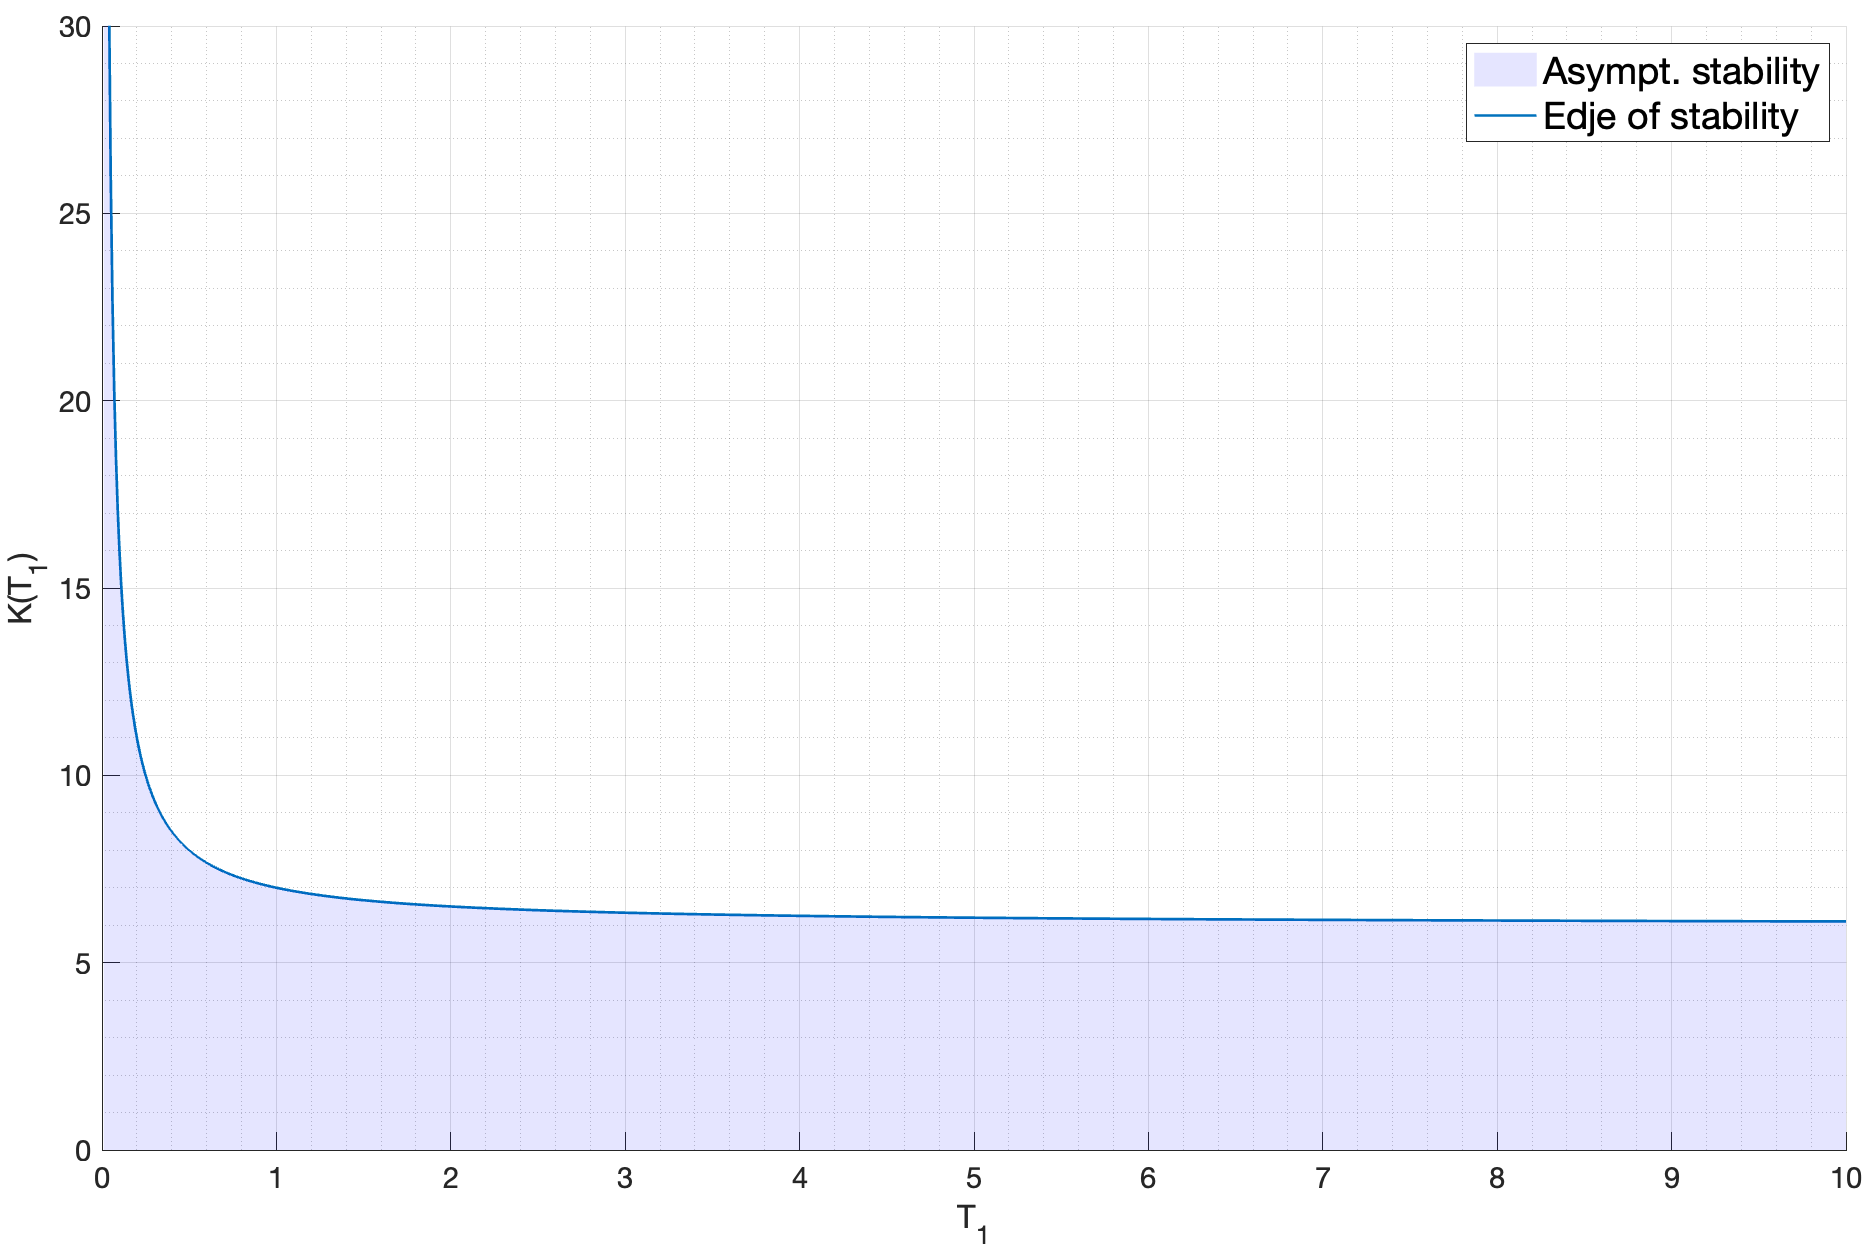
\includegraphics[width=\textwidth]{media/T1.png}
    \caption{Граница и область асимптотической устойчивости для $K(T_1),~T_2 = 2/11$}
    \label{fig:T1K}
\end{figure}

\begin{figure}
    \centering
    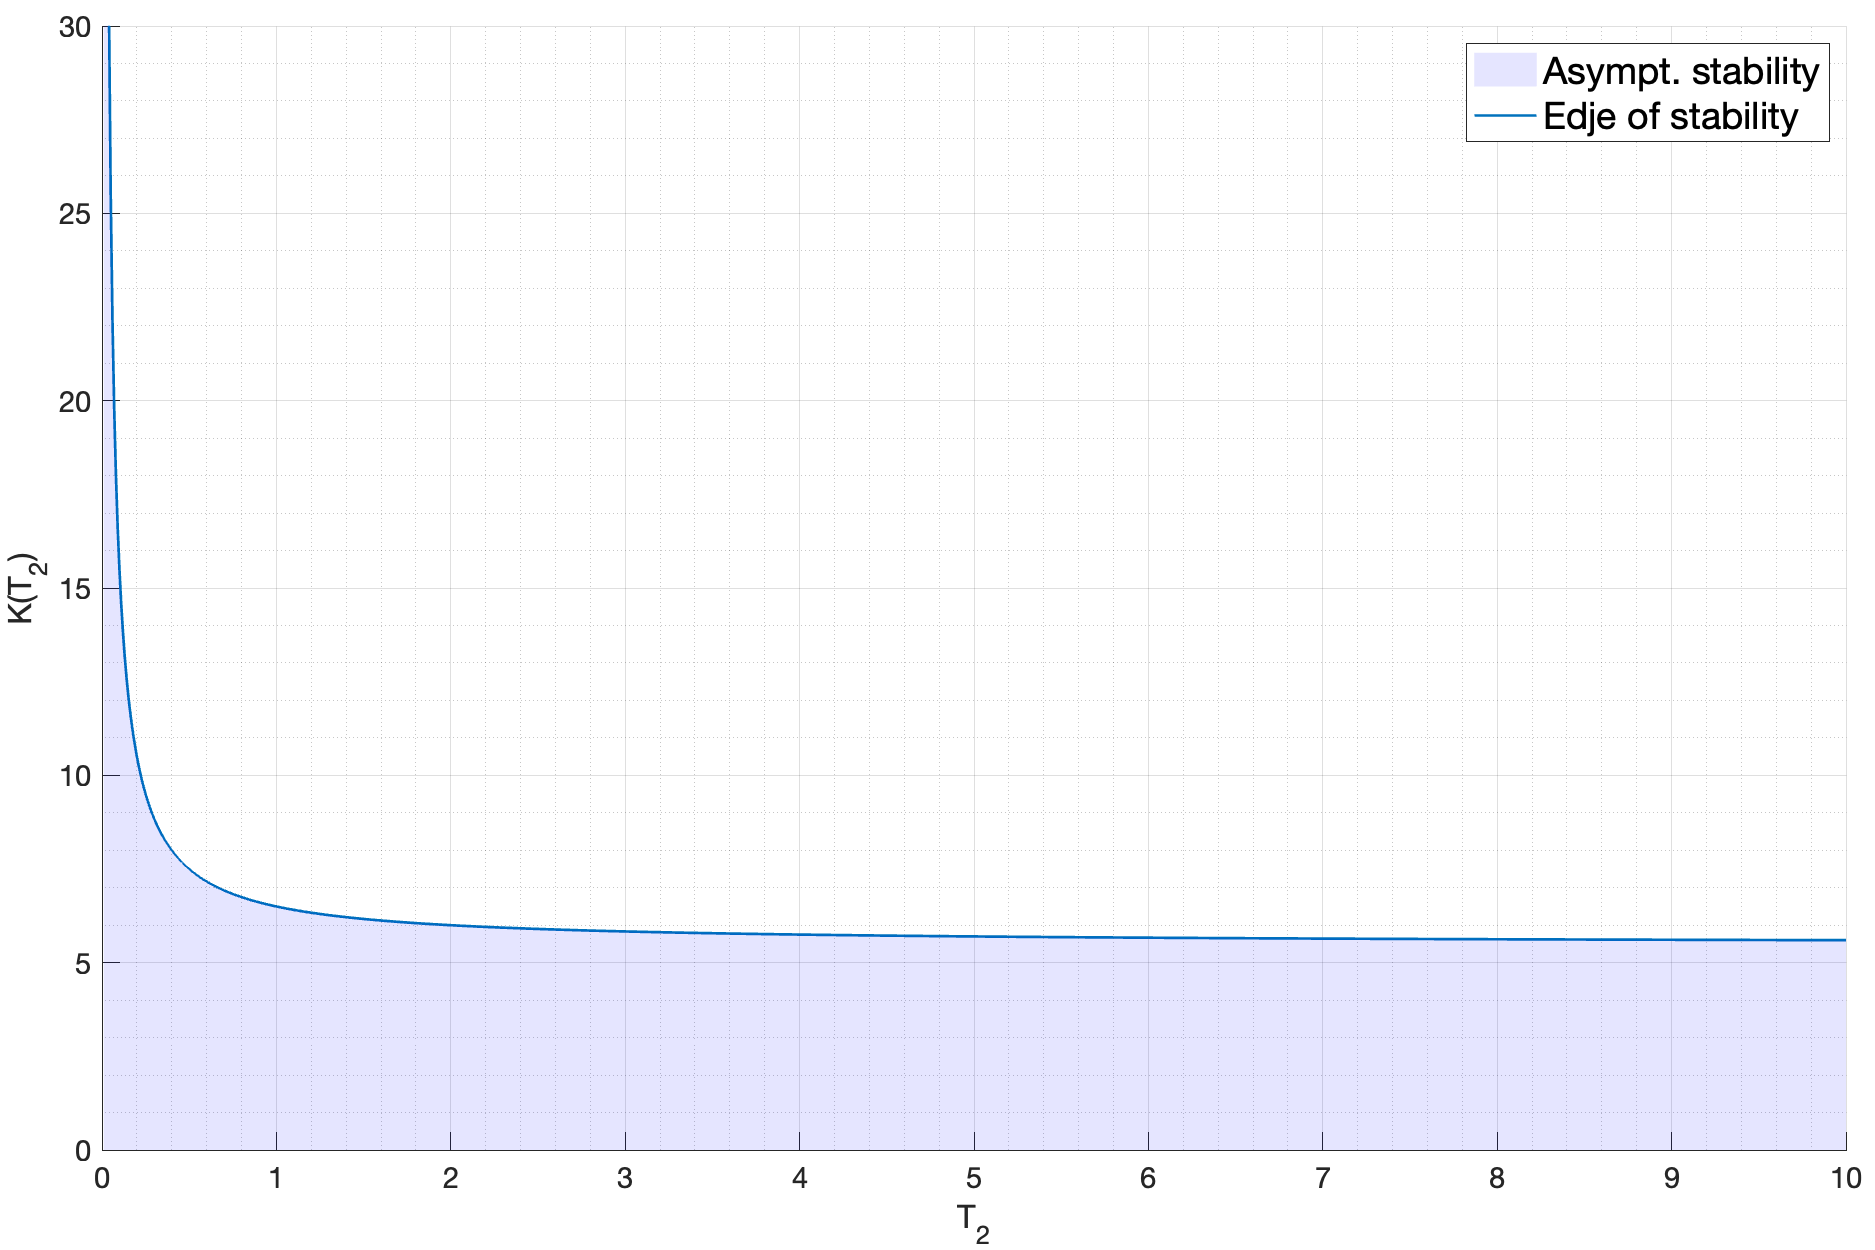
\includegraphics[width=\textwidth]{media/T2.png}
    \caption{Граница и область асимптотической устойчивости для $K(T_2),~T_1 = 1/6$}
    \label{fig:T2K}
\end{figure}

\FloatBarrier
\subsection{Моделирование}
Выберем значения, которые будет соответствовать разном типам устойчивости:
\begin{itemize}
    \item $T_1 = \frac{1}{6},~T_2 = 1,~K = 5$ -- область асимптотической устойчивости
    \item $T_1 = 1,~T_2 = \frac{2}{11},~K = \frac{13}{2}$ -- граница устойчивости
    \item $T_1 = \frac{1}{6},~T_2 = 2,~K = 10$ -- область неустойчивости
\end{itemize}
И проведем моделирование системы для каждого из случаев. Результаты моделирования приведены на рис. \ref{fig:case7} -- \ref{fig:case9}.

\begin{figure}[ht!]
    \centering
    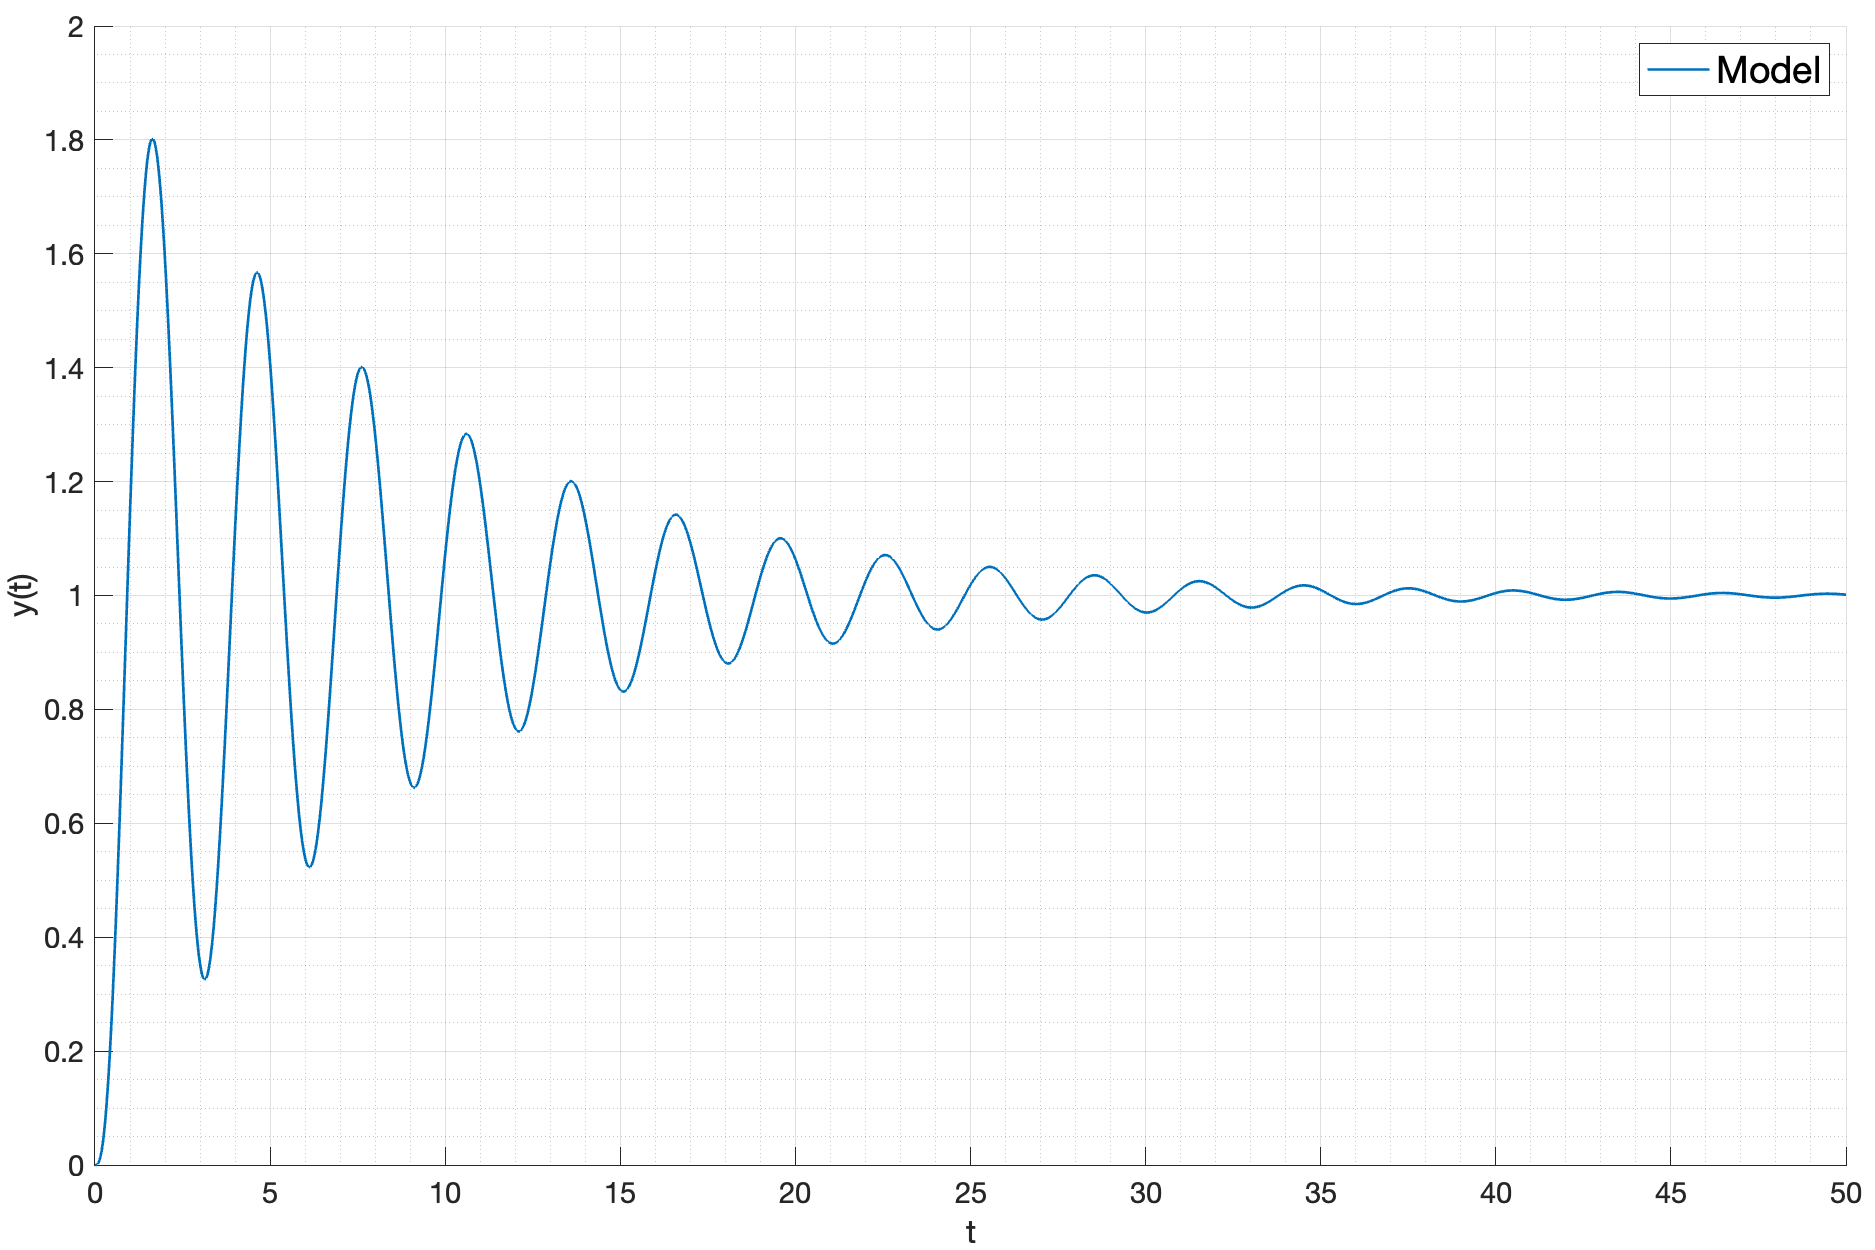
\includegraphics[width=\textwidth]{media/case7.png}
    \caption{Моделирование для области асимптотической устойчивости}
    \label{fig:case7}
\end{figure}

\begin{figure}[ht!]
    \centering
    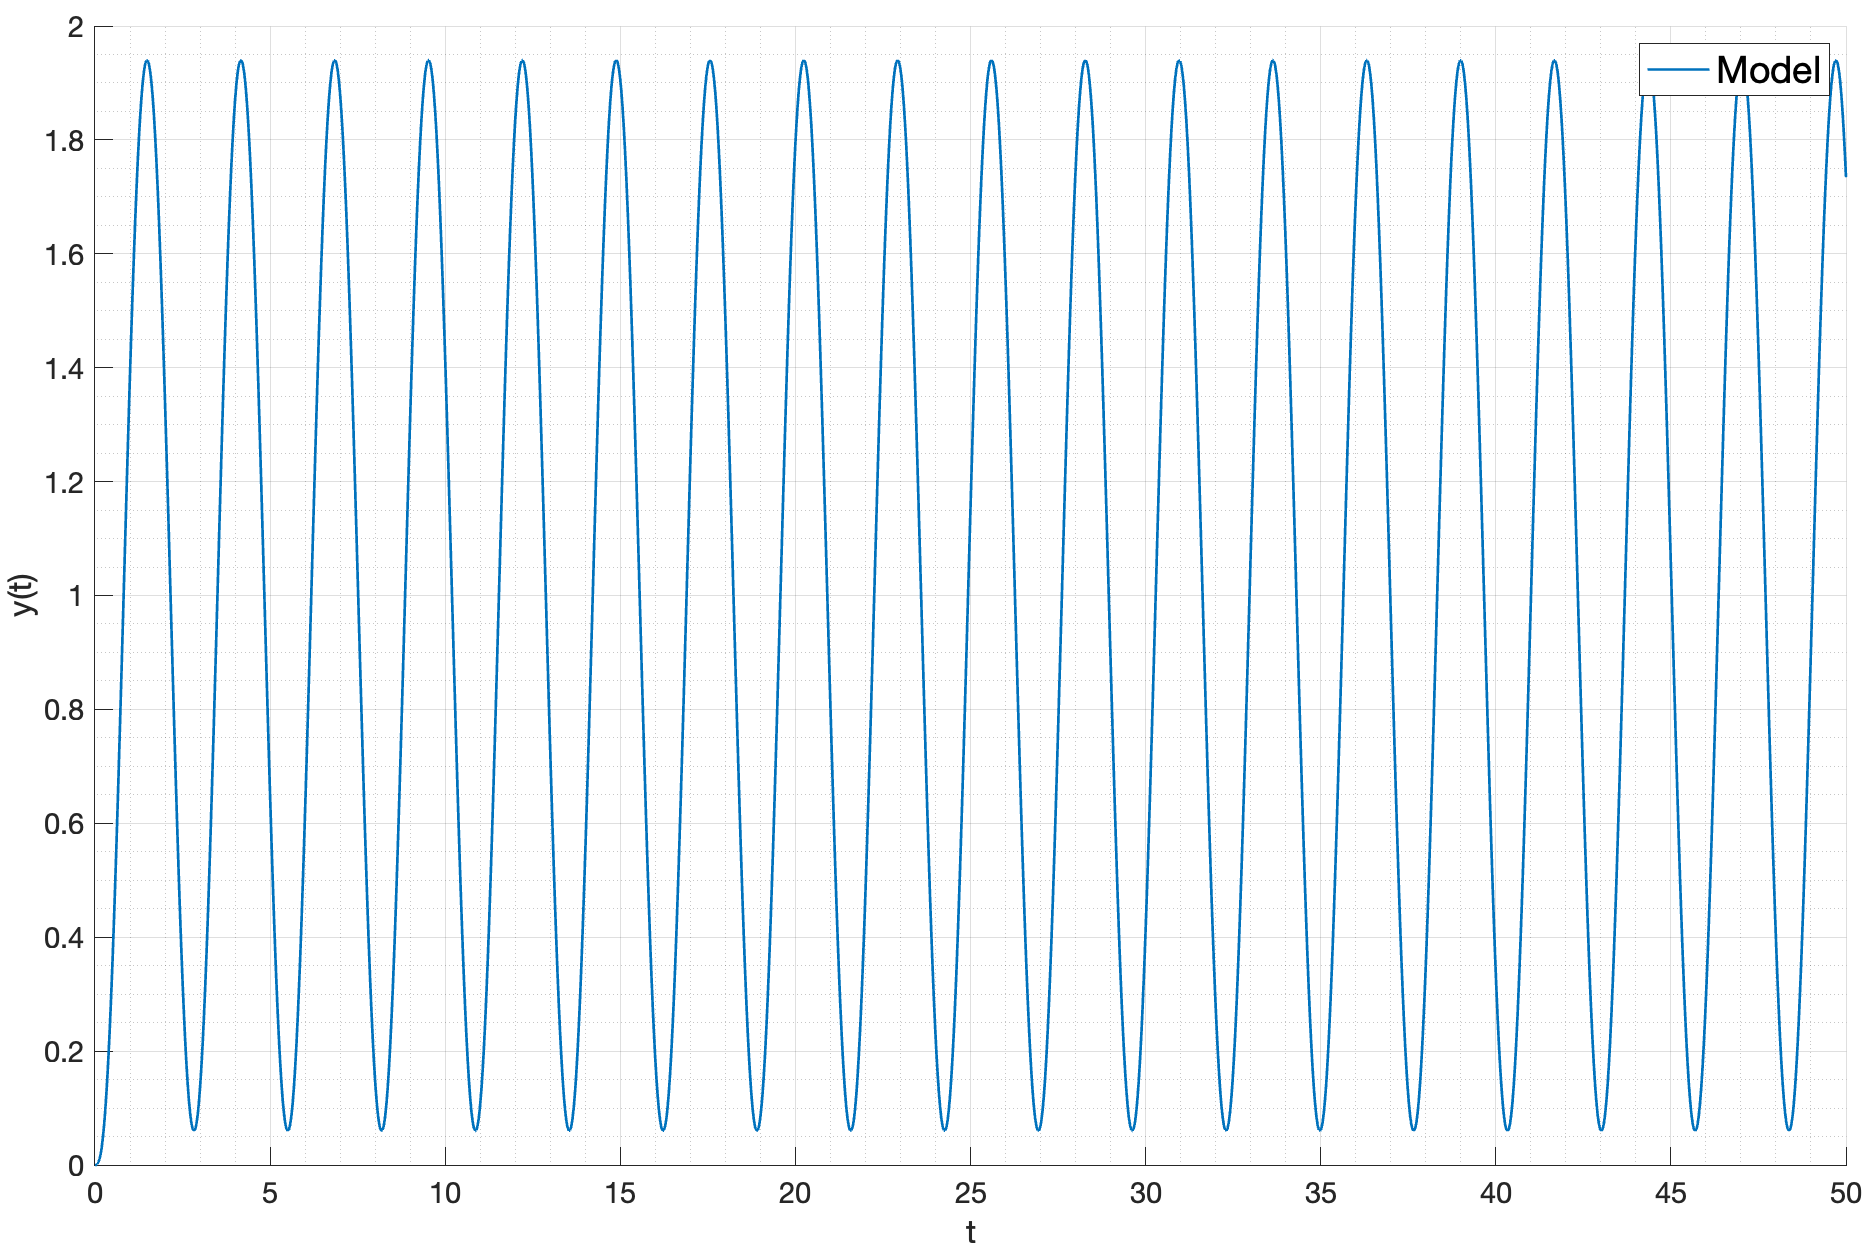
\includegraphics[width=\textwidth]{media/case8.png}
    \caption{Моделирование для границы устойчивости}
    \label{fig:case8}
\end{figure}

\begin{figure}[ht!]
    \centering
    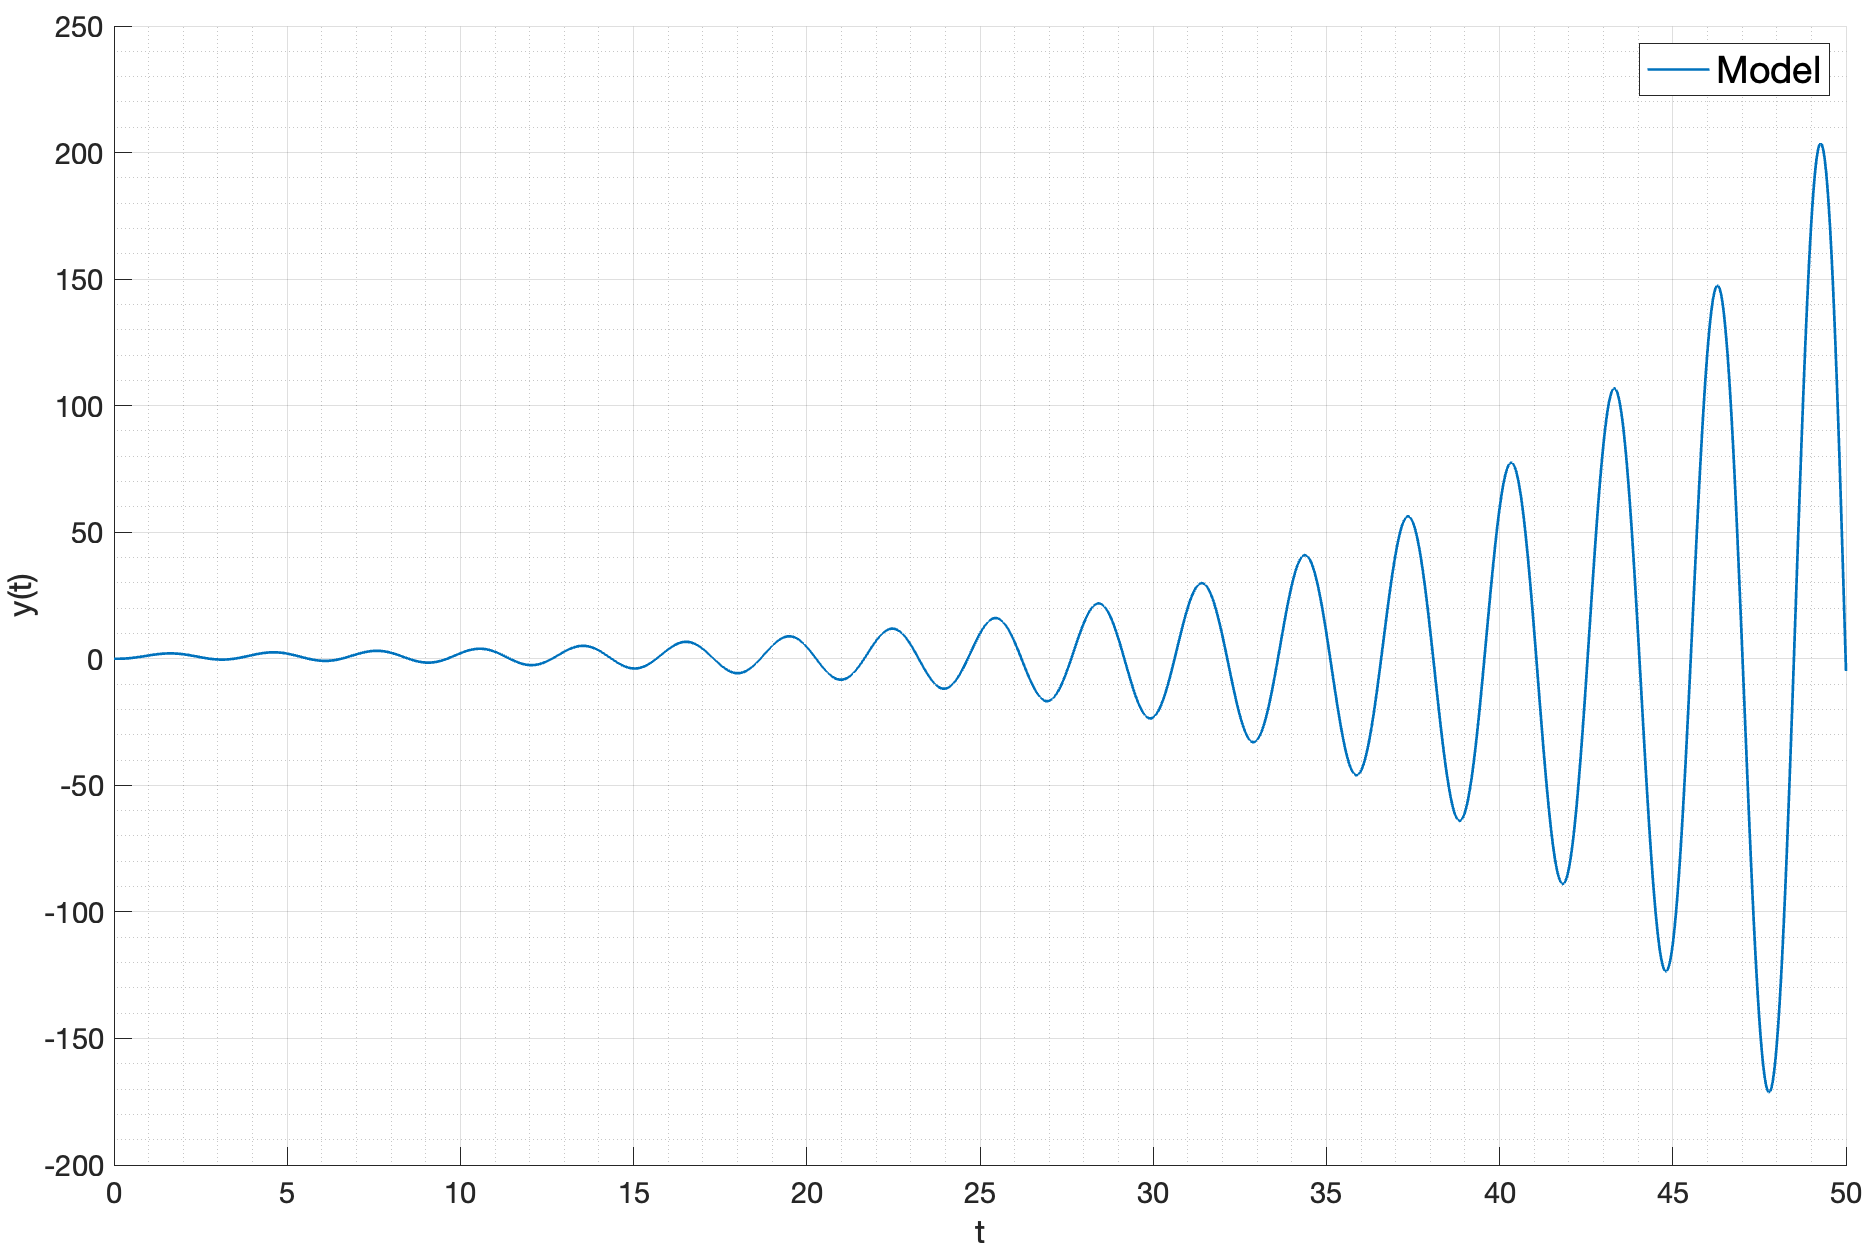
\includegraphics[width=\textwidth]{media/case9.png}
    \caption{Моделирование для области неустойчивости}
    \label{fig:case9}
\end{figure}

\subsection{Вывод}
В результате моделирования системы можно сделать вывод, 
что полученные значения $T_1,~T_2,~K$ соответствуют теоретическим ожиданиям устойчивости системы.
Это значит, что критерий Гурвица позволяет определить область устойчивости системы аналитически. 